\documentclass[proposal]{umassthesis}
\usepackage{graphicx}
\usepackage{url}
\usepackage{amsmath}
\usepackage{cite}

\begin{document}

%%
%% You must fill in all of these appropriately
\title{Mobile privacy in an untrustworthy world}
\author{Keen Y. Sung}
\date{February 2018} % The date you'll actually graduate -- must be
                     % February, May, or September
\copyrightyear{2017}
\bachelors{B.Sc.}{University of Alberta}
\masters{M.S.}{University of Massachusetts}
\committeechair{Brian N. Levine}
\firstreader{Mark Corner}
\secondreader{Joydeep Biswas}
\thirdreader{Dennis Goeckel}
\departmentchair[Chair]{James Allan} % Uses "Department Chair" as the title. To
% use an alternate title, such as "Chair", use \departmentchair[Chair]{Pete Shearer}
\departmentname{College of Information and Computer Sciences}

\degree{Doctor of Philosophy}{Ph.D.}
\frontmatter
\maketitle
\copyrightpage     %% not required for an M.S. thesis
\signaturepage
% '\newcommand{\myparagraph}[1]{\paragraph{#1}\mbox{}\\}
\begin{abstract}                % Abstract
%!TEX root = umthsmpl.tex

In this dissertation, I analyze and improve the security and performance of blockchain systems across three primary themes. In the first theme, I analyze blockchain algorithms for setting difficulty, a network parameter that controls the inter-arrival of blocks. Fluctuations in mining power can cause uneven inter-block delays when the difficulty is not set accurately.  Mining power can change due to many reasons, including the miners' allocation of hardware and swings in the exchange rate of a currency.  For example, Bitcoin Cash saw enormous variance in mining power at its creation and the algorithm for difficulty did not easily converge. Therefore, we propose and characterize two alternatives to accurately update difficulty: one that solely uses information that is currently available, and another based on status reports that are partial blocks regularly broadcasted.

Status reports add overhead into networks because they require the broadcast of additional information. In a second theme, I introduce a novel method for the propagation of status reports and blocks. We evaluate, analytically and We show that our approach, called Graphene, improves network performance by reducing the size of blocks.

In the third theme, I analyze the practical feasibility of prominent attacks, such as double spending and selfish mining, on blockchain systems. Most analyses generally assume that the mining power of honest and malicious miners is known by an attacker. However, we show that estimation of mining power introduces error into these models. Therefore, we argue that these attacks are difficult to carry out with high precision, and use reinforcement learning techniques to realistically evaluate them when an attacker does not have full knowledge of the network's mining power.

\end{abstract}

\tableofcontents                % Table of contents
\listoftables                   % List of Tables
\listoffigures                  % List of Figures

\mainmatter   %% <-- This line is mandatory

%!TEX root = umthsmpl.tex
\unnumberedchapter{Introduction}

\section*{Contributions}
The following is a summary of the contributions in each chapter of this proposal. 
%\begin{itemize}
%\item Firstly, we propose an accurate method of hash rate estimation that is based
%  on compact {\em status reports} issued by miners. The reports add no
%  computational load to miners, and are stored neither on the
%  blockchain nor at peers that receive them past their usefulness.   They are very small and  can be broadcast
%  out-of-band, for example via RSS or Twitter. Just like block
%  headers, reports are verifiable as authentic POW by third
%  parties. 
%  %Optionally, they can be used to set the blockchain difficulty, in which case they would need to be stored on the blockchain. This technique can be deployed incrementally because a combination of our estimators can be used together.
%  \item Secondly, we present two estimators that leverage only information from blocks that are published to the blockchain. One method uses {\em time} data, while the other uses time and the POW {\em hash values} of blocks. Both require {\em no cooperation from the miners}. These estimators are statistically \emph{biased} but \emph{consistent}. In quantitative comparisons, we show that the time-based estimator is more accurate. However, this accuracy depends on reliable time measurements. For example, although blocks contain timestamps, Bitcoin has weak time synchronization requirements allowing for falsification. Any third-party's out-of-band record of the time cannot be secured using  only information in the blockchain. We find that a time-and-hash based estimator is less accurate (given the same number of samples) despite leveraging more information.  
%  % via the PoW algorithm
%\end{itemize}
%We also examine hybrid approaches that allow for incremental deployment. 
%Our results can be used by blockchain designers to understand the consequences of setting the parameters of their difficulty algorithms. 

\paragraph*{1.}

\paragraph*{}

\paragraph*{}


\section*{Collaborators}
%!TEX root = umthsmpl.tex
\chapter{A model of location privacy and utility}
\label{ch1}

Many current models of location privacy primarily model threats from location based services, and propose defenses based on differential privacy strategies~\cite{andres2013geo,ho2011differential}.
However, the strategies studied in these works involve a service provider obfuscating databases of location logs, which requires the user to trust the service; this is not applicable from the point of a user who does not trust the service. 
In this chapter, I plan to generalize an existing method of quantifying location privacy~\cite{shokri2011quantifying}, and extend it to allow for threats from non-LBS usage. In my preliminary work, I present a novel framework to identify a user from both location profiling (LP) and trajectory linking (TL).
%I look at potential vectors for attacking location privacy, and argue for an economic model of privacy. I also
I propose to investigate game theoretic~\cite{freudiger2009non} and information theoretic models~\cite{sankar2013utility} to capture the varying worth of location privacy depending on the user and location. I will also evaluate the accuracy of the LP/TL framework and these models using a synthetic dataset created from a field survey. I will seek additional datasets as well.

\section{Preliminary work: Framework for location profiling and trajectory linking}
% I employ a utility model to quantify location privacy. 
I summarize the different adversaries and types of threats against location privacy. Next, I develop a general model of location profiling and trajectory linking that can be used in various ways by these attackers. Finally, I evaluate some simple location profiling and trajectory linking algorithms.
%Next, I formalize the framework behind several of these problems. I then discuss several possible scenarios and how they fit in this framework. Finally, I evaluate the risk-privacy balance with respect to a mobility dataset.

\paragraph*{Overview}

\begin{figure}\begin{center}
	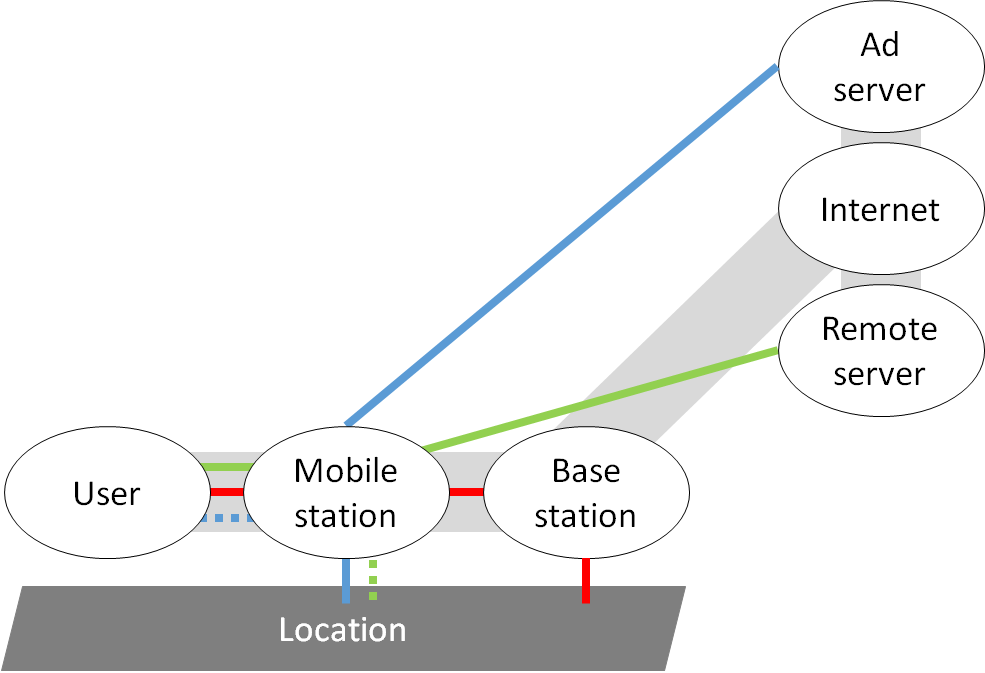
\includegraphics[width=\textwidth]{graphics/attacks}
	\caption{Exposure of information that may result in potential vulnerabilities in location privacy. The user, mobile device, and base station are in some physical location. The thick gray line indicates the communication path between a user and a service. Solid colored lines indicate links known to a potential attacker. Dotted colored lines indicate links that may be inferred by an attacker. Red lines indicate information known to a service provider; blue an advertising client; and green a web service.}
	\label{fig:overview}
\end{center}\end{figure}

There are many ways people remain connected to the Internet, such as Wi-Fi, cellular network, and cable. In each of these cases, the time and location of a user connection is known to the service provider. There have been cases of IMSI-catchers being used dubiously to monitor individuals~\cite{dabrowski2014imsi}. Additionally, passive eavesdropping techniques may intercept any mode of wireless signal, including Bluetooth, allow for a varying degree of granularity to localize an individual. We need a flexible framework to model these types of attacks. Such a framework would allow us to measure and quantify wireless geolocation privacy with varied settings and attacker models. 

There are many attack vectors on a user's location privacy. Figure~\ref{fig:overview} diagrams the potential vulnerabilities from different classes of attackers. In Chapter~2, I look at a web service attacker. This service has information about who the user is and which device she is using, and may infer the location of the device (green lines). In Chapter~3, I look at advertiser attackers, who have information about the device's location, and may infer who the user is (blue lines). In Chapters 4 I look at service provider attackers, and how to defend against them. These attackers have concrete information about the user, device, and location, so we must break the link between user and device (red lines). 

The following is a general framework that uses trajectory linking to improve location profiling. For simplicity, the following equations do not take into account the time of day, and other factors that may help determine the user of a trace. It contains no details about the location profiling and trajectory linking themselves.

\paragraph*{Model}
Let $U$ be the users in our database. These are users for which we have some location history data $S_U$.
Let $S^*$ be all sequences of locations $L$ within some time range of interest.
A sequence $\mathbf{s}\in S^*=s_0,\dots; s_i\in L$.

The most likely user given an anonymous sequence of locations is
\begin{equation}
\arg\max_up(u|\mathbf{s}),
\end{equation}
where 
\begin{equation}
p(u|\mathbf{s}) = p(u|s_0,\dots).
\end{equation}

We can determine the most likely path for a user as
\begin{equation}
\arg\max_\mathbf{s} p(\mathbf{s}|u).
\end{equation}

Trajectory linking is the most likely sequence given another sequence:
\begin{equation}
\arg\max_\mathbf{s} p(\mathbf{s}|\mathbf{s'}).
\end{equation}

Finally, we can determine the most likely user of a sequence using information from possible additional trajectories. 
Let $Z^s$ be the permutation of paths in $S^*$ that are linkable to $s$ (i.e., there is no overlap in time, and no impossibly fast transitions), then
\begin{equation}
p(u|\mathbf s) = \sum_{z\in Z^{\mathbf s}} p(z|\mathbf s) p(u|z).
\end{equation}
Generating a permutation of paths and computing their probability is intractable for many tests, so we may use heuristics to include only obvious links.

If an attacker wishes to deanonymize an entire anonymized database, they would want to determine the most likely matching of users to traces. 

We can determine the most likely corresponding (ordered) set of users $\hat{U}$, given some set of anonymous traces $S^{*'}\subseteq S^*$ as
\begin{equation}
\arg\max_{\hat{U}} p(\hat{U}|S^{*'}),
\end{equation}
where
\begin{equation}
p(\hat{U}|S^{*'}) = \prod_i p(\hat{U}_i|S^{*'}_i).
\end{equation}

To determine a set of users, given some anonymous set of traces, and consider possible links, we calculate
\begin{equation}
p(\hat{U}|S^{*'}) = \prod_i \big( \sum_{z\in Z^{S^{*'}_i}} p(z|S^{*'}_i) p(\hat{U}_i|z) \big).
\end{equation}

Accordingly, the $k$-anonymity of a user $u$, given a trace $s$, is 
\begin{equation}
k\textrm{-anonymity} = \textrm{rank}(\langle p(u|\mathbf{s}), u \rangle, U).
\end{equation}

\paragraph*{Linking algorithms}

There are effective, naive location profiling algorithms~\cite{de2008identification}. A simple location profiling algorithm can effectively determine the users of anonymous sequences. In the Reality Mining dataset~\cite{eagle2006reality}, 95 anonymous users could be deanonymized with 80\% accuracy (as I show in Chapter 4). % TODO: existing experiments with motifs
However, most trajectory linking algorithms have been intended for improving positioning or object tracking, rather than from an adversarial perspective~\cite{jaqaman2008robust,yang2012online,qin2012improving}. I investigate some trajectory linking strategies in this section.

I evaluated two methods of linking using traces of 300\,000 cell phone users in a particular country\footnote{I was unable to obtain permission to publish using this dataset; thus, I have abandoned these results, and will have to find an alternative for my thesis.}, tracked two weeks at a time. Each user had a log of which location area code (LAC) among 1\,666 they were present in every ten minutes.

\emph{Motifs.} Because the dataset had only 1666 LACs, the mobility data was very coarse. This means that our traces do not capture much mobility unless a user makes distant trips. I was unable to regular sequences of paths that are more than three locations. Among 100000 users, I was able to identify paths with 3-location trajectories linked once with another (6 locations long) with 40\% accuracy. Note that the existence of these trajectories were exceptionally sparse in this dataset.

\emph{Estimated link frequency.} To estimate the likelihood of a link occurring, we count the frequency of a link (i.e. a transition from location $a$ to $b$) in the dataset. 
Assuming
\begin{align}
	Count(AppearsTogether(a,b))&=Count(a) + Count(b),\label{eq:link}\\
	\textrm{then } E[p(a\rightarrow b|a,b)] &= \frac{Count(a\to b)}{Count(a)+Count(b)}\label{eq:link2}
\end{align} 

However, it may be the case that $a$ and $b$ rarely appear together (in time). For example, $a$ may appear a lot more than $b$, but $b$ often transitions from $a$. This breaks the assumption in Equation~\ref{eq:link}. We can make the assumption that the probability $b$ comes from $a$ and $a$ goes to $b$ is similar when they appear together as when they do not, in which case, we have 
\begin{align}
\label{eq:link3}
	E[p(a\rightarrow b|a,b)] &= \frac{p(a|b)*p(b|a)}{p(b)*p(a)}
\end{align}
% TODO: fix this, maybe

The results from this linking method is shown in Figure~\ref{fig:linkcdf}.
\begin{figure}\begin{center}
		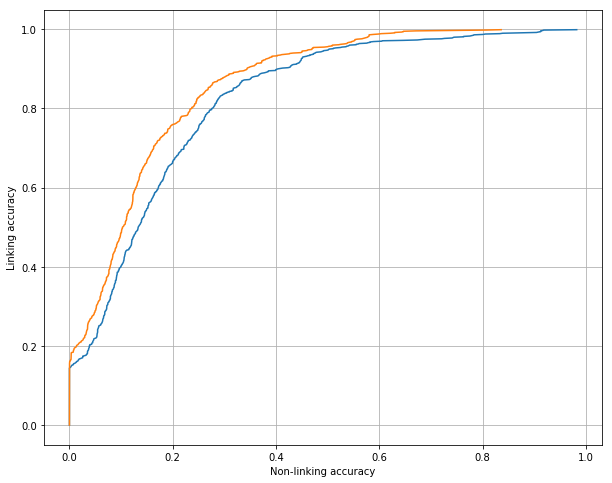
\includegraphics[width=0.7\textwidth]{graphics/linking2}
		\caption{The $x$-axis represents accuracy of identifying a set of traces unlinked, and the $y$-axis represents the accuracy of the same set linked based on Equation~\ref{eq:link3}. Red is a link before, and blue is a link after.
		\label{fig:linkcdf}}
\end{center}\end{figure}

% TODO: better caption or label
\begin{figure}\begin{center}
		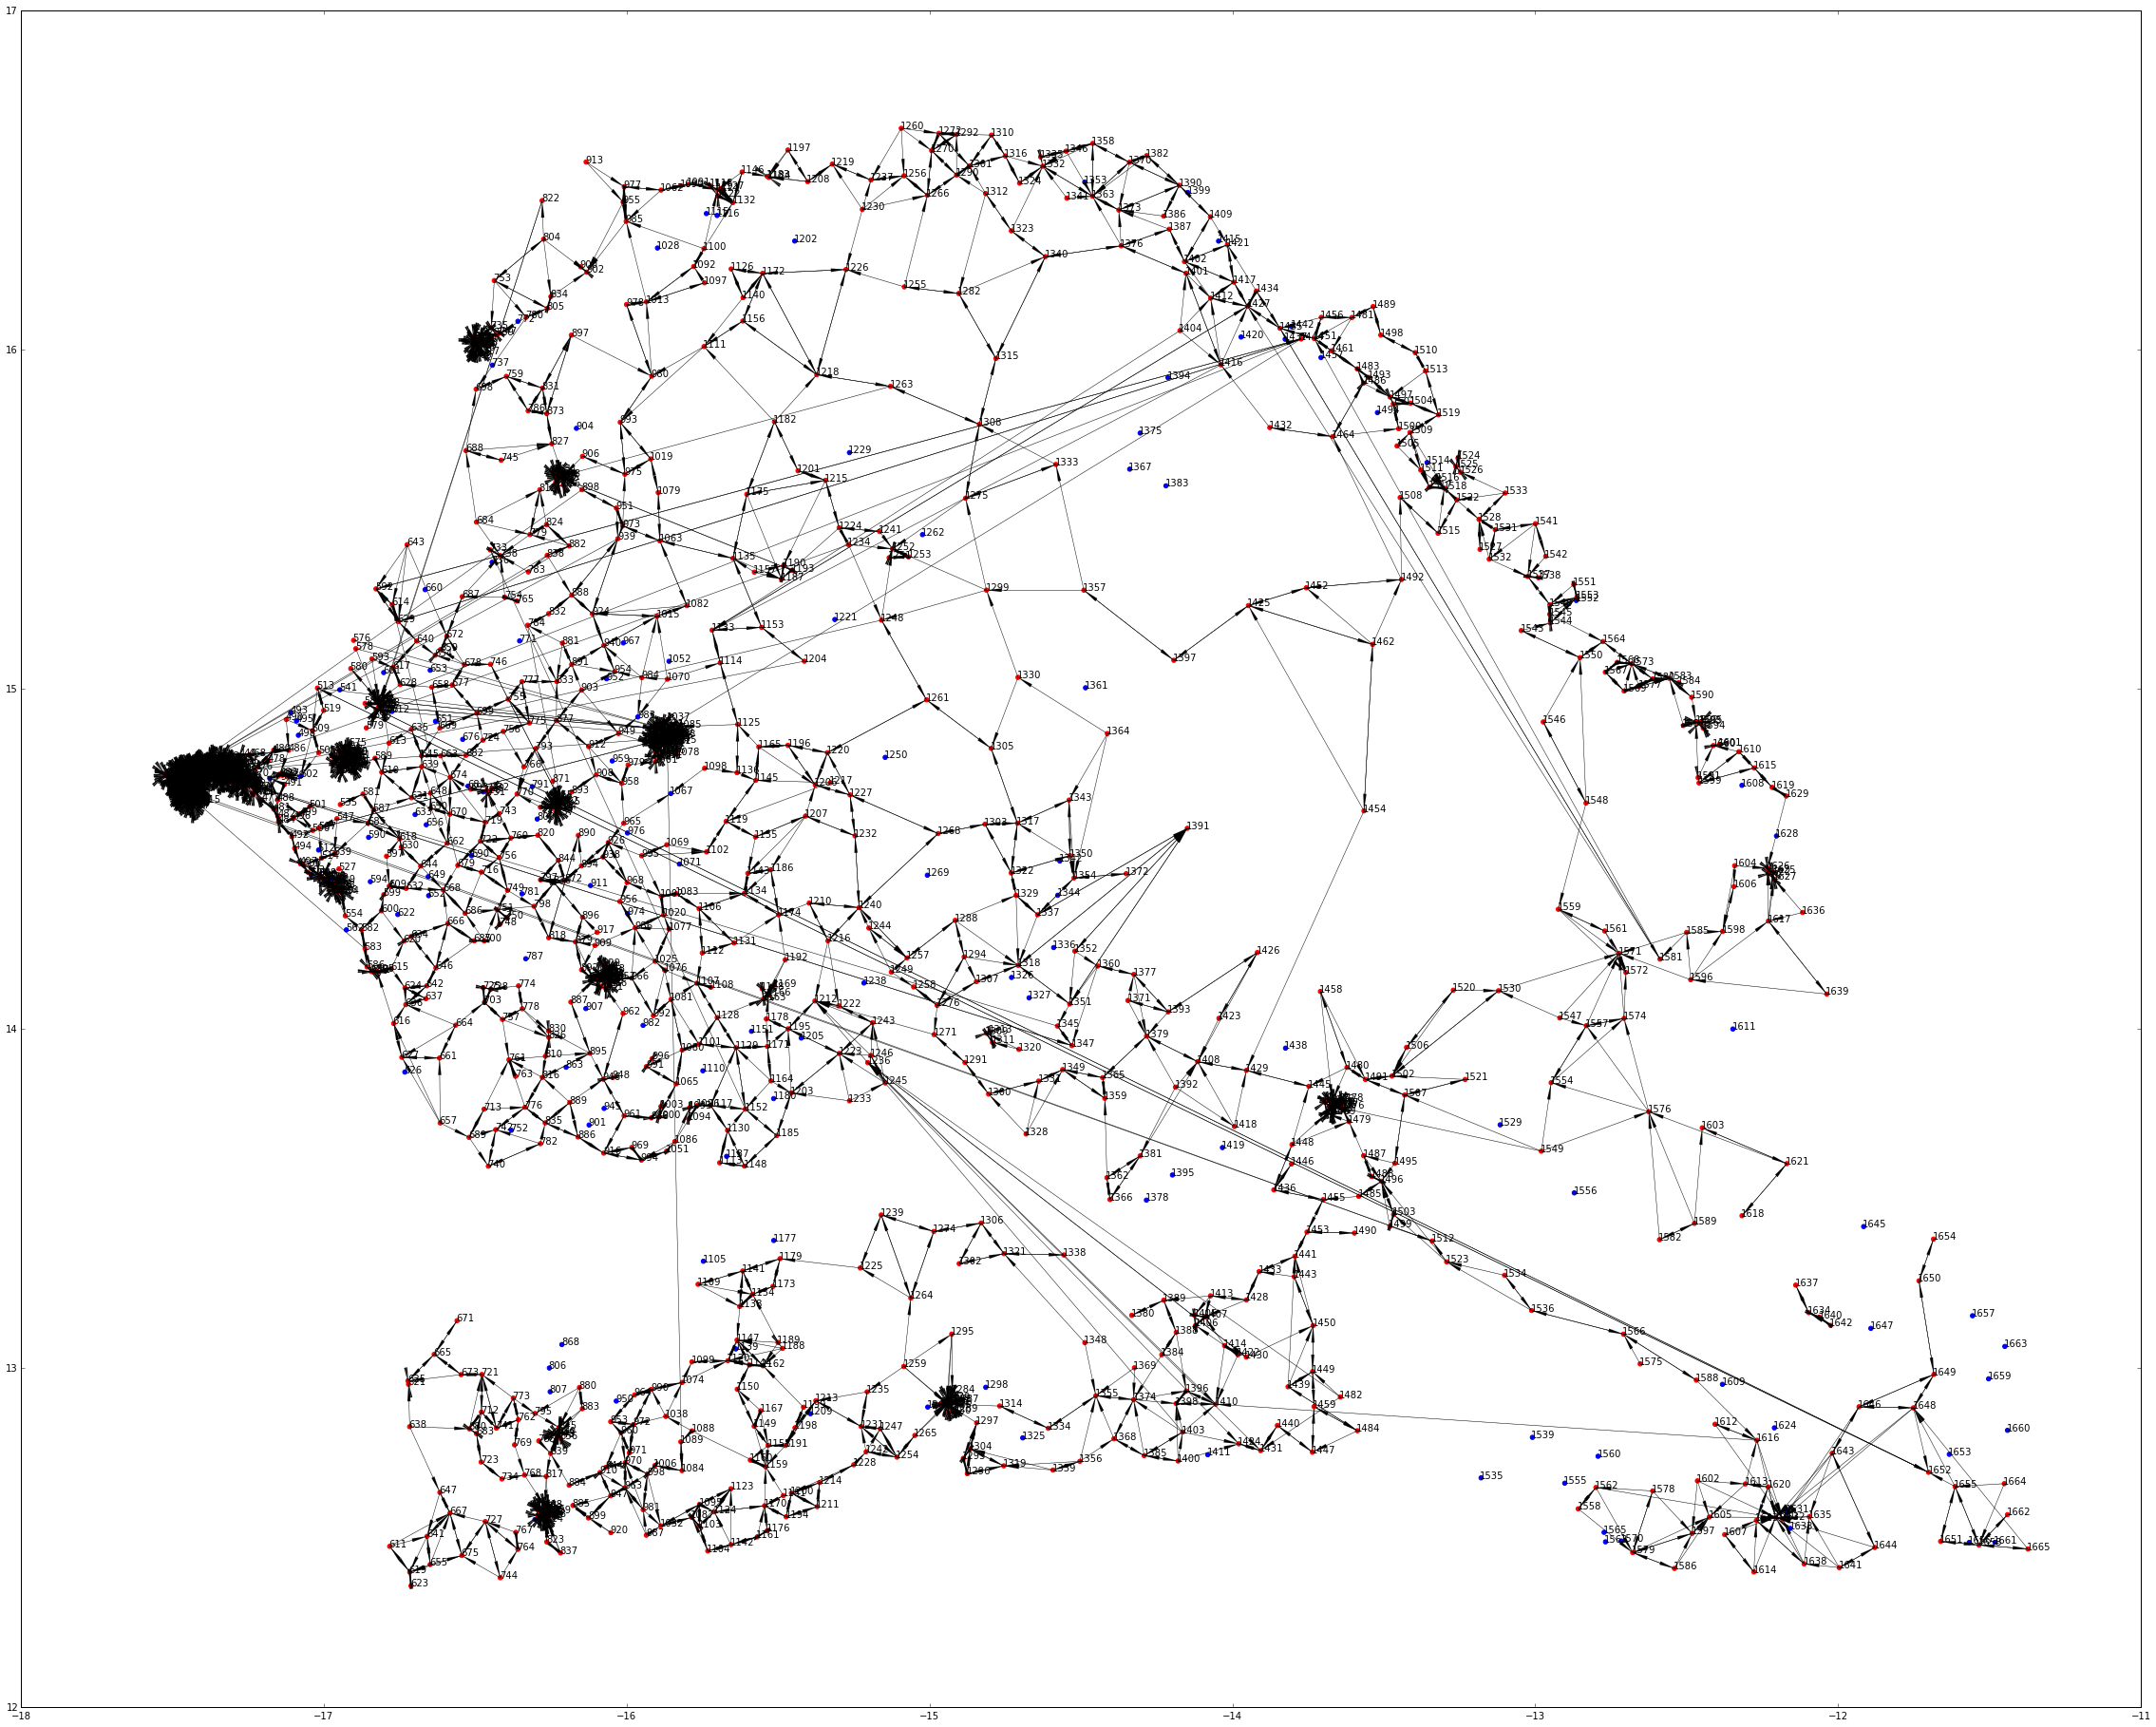
\includegraphics[width=\textwidth]{graphics/senegalmap}
		\caption{Most common LAC transitions in Senegal. Longer lines may indicate trips by air or sea.
			\label{fig:senegal}}
\end{center}\end{figure}

Multiple target tracking (MTT) algorithms\cite{nillius2006multi} can be used as heuristics for trajectory linking. Because the dataset above contains only coarse data on time and physical location, MTT would be ineffective. To simulate the finer-grained location data that a cell tower would have, I use a dataset tracking over 300 taxis in the Rome metropolitan area over a month\cite{cunha2015understanding} to evaluate the effectiveness of a naive MTT algorithm\footnote{\url{http://soft-matter.github.io/trackpy}} for trajectory linking, assuming no points are linked initially. Figure \ref{fig:mtt} shows that if location is updated constantly, taxis would still be identified with 40\% accuracy without any initial linking.

% TODO: self mixing, breaking links

% TODO: fix legend --- area of thing
\begin{figure}\begin{center}
	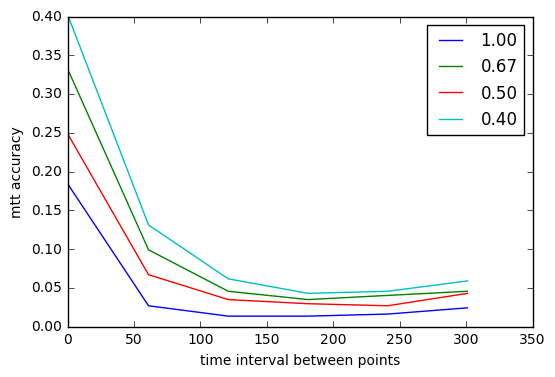
\includegraphics[width=0.7\textwidth]{graphics/mtt}
	\caption{MTT accuracies for 374 taxi drivers around Rome over a period of 20 minutes. Colors represent different relative granularities.}
	\label{fig:mtt}
\end{center}\end{figure}

%% TODO: stuff for Mariya
%% TODO: linking algo for the D4D data


\section{Proposed work: Fully implement a utility model and collect data to rigorously evaluate it}
%\paragraph*{Utility-privacy framework}

I was able to pilot trajectory linking and location profiling using several datasets; however, these datasets are insufficient to evaluate any algorithm (and one has not given us permission to publish). Additionally, many datasets are either old, crowd-sourced, or have been fuzzed with noise. To extend this chapter, I propose to answer a few key questions:
\begin{enumerate}
	\item What are some properties of the wireless topology on a cell phone network in a rural or urban area? Knowing these properties would allow me to more accurately synthesize and validate a dataset.
	\item How effective are LP/TL algorithms in de-anonymizing traces?
	\item What is the utility cost to avoid being tracked by these algorithms?
	% \item What is the efficacy and complexity of LP/TL methods?
	% \item How effective are these methods after excluding low-value locations such as home and work?
	% \item How useful is information about wireless topology in LP/TL algorithms?
\end{enumerate}

To answer these questions, I will first do field surveys of the Amherst and Boston areas, to determine the density of cell towers and physical locations served. If I am able to recruit enough users, I will track how often a phone connects to the network to make a call. The call data in particular will be useful in Chapter~4. 

Using this information, I will synthesize a larger dataset of mobility traces and calls, and validate this against any additional datasets I find. I will use these datasets to develop and evaluate several location profiling or trajectory linking algorithms. 

Finally, I plan to develop a model to measure the balance between utility and privacy. I will alter traces in the aforementioned datasets to simulate evasive reduction of phone usage, and analyze the trade-off between usability and privacy. I will pay special attention to how much significant stays like home or work may make a use significantly more identifiable, but is information that is of little value to both targets and attackers. An economic model may better encapsulate these possibilities, if a user can assign different values to different locations.

% Previous work has used $k$-anonymity, or $(k, p)$-anonymity as a privacy metric\cite{shou2013supporting}. Instead, we use the economic measure of utility as a metric for two reasons: (1) it allows us to balance the cost of utility with the cost of privacy loss, and (2) it allows us to assign different values to different locations. For example, a user could have "significant stays" at home and work, a place where they would likely be identified, anyway, so achieving location privacy here is not worth it if they are able to change identities without being easily linked once they leave work.

% I plan to adapt the framework above for use in an economic model of privacy, as well as compare it against other known models for privacy\cite{shokri2011quantifying,shin2012privacy}. I plan to implement more sophisticated location profiling and trajectory linking algorithms to work with the framework. I will also do a field survey by sending phones around the Amherst area and collecting information about cell phone towers, signal strength topology, and synthesizing a dataset to evaluate these algorithms. 
%!TEX root = umthsmpl.tex
\chapter{Location privacy threats from a streaming service}
This chapter explores the threats to location privacy when a user downloads data while in motion, and presents an evaluation on the loss of utility if a user attempts to reduce these threats\footnote{This chapter is based on work published at the Privacy Enhancing Technologies Symposium\cite{soroush2013turning}}. I propose to analyze in more detail some algorithms more suited to this problem, and the trade-offs between traffic-shaping to preserve privacy and utility.

\section{Preliminary work: Identifying the path traveled using throughput}

Despite features on smartphones to ensure location privacy, a user's whereabouts can be remotely deduced. A remote party communicating with a phone has a window into the complex interactions between phone and cell tower. These features can be used to reveal the phone's location, or at least significantly narrow the list of possible paths taken by a phone and its owner. This information is leaked regardless of application-level privacy settings. Cell phone users have such experiences intuitively in many common situations. For example, a caller may be able to tell when a friend has entered an elevator based solely on call quality; or a user may notice a loss in data throughput during a subway ride.

We collected hundreds of traces of music that we streamed to 
phones along four geographically separate routes in two 
directions each.  We find that within small geographical areas,  
mean throughput is largely consistent and distinct. We examine 
the accuracy of three
remote localization classifiers that leverage this consistency. 
Even a naive approach, trained on the mean throughput of each path, 
has some success. 
We compared this classifier against a
$k$-nearest neighbors ($k$-NN) classifier, which trains on the ordered
sequence of throughput values of each rout, a hidden Markov model
(HMM) classifier, which exploits the consistency in throughput values
at each location, and a Naive Bayes (NB-KDE) classifier that uses
kernel density estimation of throughput at each second along a path.
Our best performing approach, the NB-KDE classifier, can correctly
determine with greater than the path taken by the phone from one of
four longer paths to neighboring suburbs with greater than 90\%
accuracy, and the path and direction (8 choices) with 76\%
accuracy. In a separate experiment involving data collected only from
within a 4km$^2$ area, in and around our campus, the NB-KDE approach
could identify the direction and part of campus the user was traveling
with 76\% accuracy.

\paragraph*{Data}
Our measurements\footnote{Traces from our experiments are available for download from \url{http://traces.cs.umass.edu}.}
are based on four Android cell phones instrumented to record traces of GPS location and 
signal strength. %, and tower association.  
A server in our building streamed music 
continuously to the phones during measurement trials. We logged TCP traces at the server during trials. We later combined sets of corresponding phone and server traces, synchronizing by the timestamps within the traces. 

\begin{itemize}
	\item {\bf Mobile 3G Measurement Set --- Paths to Towns}: We used four phones connected to the AT\&T UMTS (3G)
	network to record traces. We collected data during a
	one-month period under varying traffic and weather conditions. Each
	measurement was taken as a phone traveled along one of four routes
	going either toward or away from our central location (point X in
	Figure~\ref{fig:map}). In total, we recorded 286 traces in
	this set.
	\item {\bf Mobile 3G Measurement Set --- Paths within Campus}: We
	recorded 141 traces from the same phones, along one of two
	directions around a bus loop on campus. Traces were collected over a
	period of eight months.
	\item {\bf Stationary 3G Measurement Set}: We recorded 29 traces from
	stationary phones, connected to the UMTS (3G) network, located in
	different locations near our central location.
\end{itemize}

\begin{figure}%[p]
	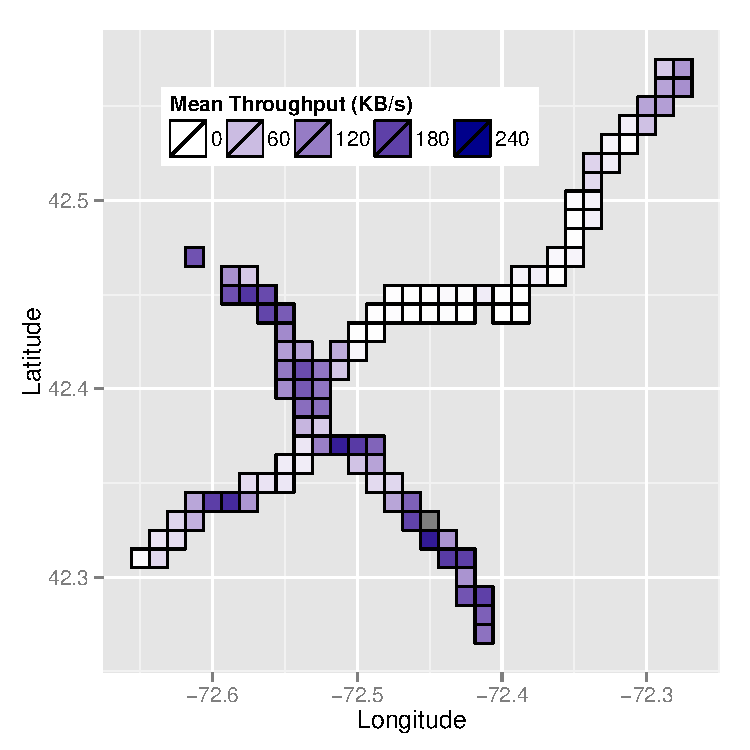
\includegraphics[width=0.5\textwidth]{graphics/amherst_tput_map.pdf}
	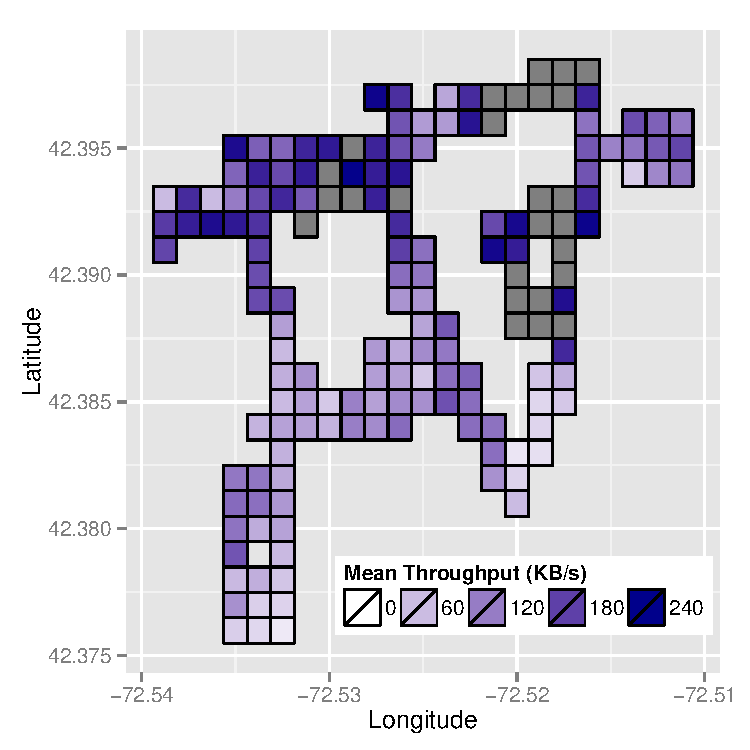
\includegraphics[width=0.5\textwidth]{graphics/umass_tput_map.pdf}
	\caption{The mean throughput of locations around Amherst (left) and
		within UMass (right). 95\% of areas have means that are statistically different from at least 90\% of other areas. This data suggests that latent information linking throughput and geography is available for training a classifier. }
	\label{fig:map}
\end{figure}

\paragraph*{Algorithms}
I present a hidden Markov model (HMM), $k$-nearest neighbors ($k$-NN),
and naive bayes (NB-KDE) classifier with respect to a motion-throughput
model. Each classifier is derived from this model, with different assumptions. The HMM classifier is most general, and attempts to maximize the estimated hidden states and transitions. The $k$-NN and NB-KDE classifiers are more rigid, and make the assumption that users move through a certain path with consistent velocity. The $k$-NN classifier finds
$k$ of the closest traces by comparing the throughput at each time
point of the trace. The NB-KDE classifier determines the distribution
of throughputs at each time point for each path, and finds the most
likely trace.

In our evaluation, we tested the identification of a path rather than
a sequence of locations. Therefore, we have split the location sequences
into separate path classes. 

For the HMM, The states are fixed as approximate square areas on the map. Emission
probabilities at each state are determined by counting the number
of occurrences of each throughput level in the training data in each
area and normalizing. A throughput level $e=0\dots15$ for 16 throughput
levels. The probability of a certain throughput level occurring at
a certain location is from a categorical distribution:

\begin{equation}
p(e|l)=\sum_{j\in N_{l}}[\mathcal{M}(o_{j}^{l})=e]/N_{l},
\end{equation} where $\mathcal{M}$ maps a throughput value $b$ to an emission level $e$ depending on which fixed range it is between.

The Markov assumption~\cite{markov1957theory} allows us to consider the probabilities of each transition independently: 
\begin{align}
p(\mathbf{l}|\mathbf{b})&=p(l_{0}|b_{0})p(l_{1}|b_{1},l_{0}),p(l_{2}|b_{2},l_{1},l_{0})\dots\\
p(l_{t}|b_{t},l_{t-1},l_{t-2},\dots,l_{0})&=p(l_{t}|b_{t},l_{t-1})\\
p(\mathbf{l}|\mathbf{b})&=\prod_{t}p(l_{t}|b_{t},l_{t-1})\\
p(\mathbf{l}|\mathbf{b})&=\prod_{t=1}^{|\mathbf{b}|}p(l_{t}|l_{t-1})p(b_{t}|l_{t})
\end{align}

For the sequence-based $k$-NN and NB-KDE, we assumed that subjects travelled
along the path at consistent speeds. Recall that for the $k$-NN and
NB-KDE, $\mathbf{c}=l_{0},l_{1},\dots$ represent a virtual location
for each second along a path, rather than directly mapping to a geographic
location.

For the $k$-NN, we compute a distance between the test trace $\mathbf{b}$
and training traces $\mathbf{b}^{tr}\in B^{tr}$, as
\begin{align}
\mathrm{distance}(\mathbf{b},\mathbf{b}^{tr})=\sum_{t=0}^{|\mathbf{b|}}|\mathbf{b}_{t}-\mathbf{b}_{t}^{tr}|.
\end{align}

Subsequently, we rank the sequences $\mathbf{b}^{tr}$ by the computed
distance from lowest to highest. We classify the instance as the label (i.e., the route) present in the largest 
fraction of the $k$-nearest neighbors. If there is a case of a tie,
we increment $k$ for that case until the tie is broken.

For the NB-KDE classifier, we determine
\begin{align}
\arg\max_{\mathbf{c}}p(\mathbf{c}|\mathbf{b}).
\end{align}

\noindent
Each location is associated with a kernel density estimator, with
Gaussian kernel $K$:
\begin{align}
f(b|l)=\frac{1}{N_{l}}\sum_{i=0}^{N_{l}}K(b-b_{i}^{l})
\end{align}

\noindent
We use the KDE to estimate the probability of a certain bandwidth
at a location, so that
\begin{align}
p(b_{t}|l_{t})=f(b_{t}|l_{t}).
\end{align}
Therefore,
\begin{align}
\arg\max_{\mathbf{c}}p(\mathbf{c}|\mathbf{b})=\arg\max_{\mathbf{c}}\prod_{t=0}^{|\mathbf{c|}}f(b_{t}|l_{t}^{\mathbf{c}}).
\end{align}

\paragraph*{Evaluation}
We evaluated the classifiers above with different scenarios using 3-fold cross-validation for hyperparameters, and leave-one-out cross-validation during training. In general, the NB-KDE classifier performed the best. The HMM classifier performed poorly, because the errors in predicting speed variations propagate as the trace gets longer. Results for every experiments are shown in Table \ref{table:mobile-accuracy}.

\begin{table}
	\centering
	\begin{tabular}{lcccccc}
			\hline {\textbf{Experiment}}&
			{\textbf{Classes}}&
			{\textbf{NB-KDE}}&
			{\textbf{k-NN}}&
			{\textbf{HMM}}&
			{\textbf{Tput}}&
			{\textbf{Freq}}\\
			\hline \hline
			4 paths$\times$ 1  (Outward)   & 4 & {\bf 90.3} & 51.4 & 18.8 &7.3 &36.6\\
			4 paths$\times$ 1  (Inward)    & 4 & {\bf 83.3} & 43.9 & 42.4 & 3.7 &28.6\\\hline
			4 paths (Western MA)$\times$ 2 & 8 & {\bf 75.7} & 25.4 & 26.1 &1.7&20.4\\\hline
			2 paths (UMass)$\times$ 2      & 4 & 75.8 & {\bf 77.6} & 53.3 &12.4& 44.7\\
			\hline
	\end{tabular}
	\caption{Classification accuracy depending on which roads are included in the experiment. Bolded entries have the highest accuracy.}
	\label{table:mobile-accuracy}
\end{table}

The NB-KDE classifier performed relatively well with short traces, as shown in Figure \ref{fig:tputlen}. Both the $k$-NN and NB-KDE classifiers increased in accuracy as length increased. This shows that while decreasing the length of the connection to the server does increase user privacy, it may not be enough; other traffic shaping options should be explored. 

\begin{figure}
	\centering
	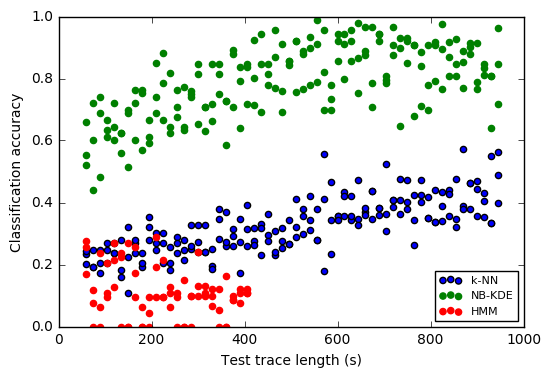
\includegraphics[width=0.7\textwidth]{graphics/tputlength}
	\caption{Accuracy of experiments (randomized test set) with varying trace lengths.}
	\label{fig:tputlen}
\end{figure}

% \section{Proposed work: Additional classifiers, and utility analyses}
\section{Proposed work}
I do not propose additional work for this chapter, though in my final dissertation, I will include a version of the work to be submitted to a journal that is more detailed than both this summary and the version presented at the \emph{Privacy Enhancing Technologies Symposium}.
%I propose to extend this work to by using more sophisticated classifiers, namely a hidden semi-Markov model \cite{johnson2013bayesian}. As well, I would use the data collected for Chapter 1 to determine the usefulness of features such as time of day (see Figure \ref{fig:tod}). Finally, I will evaluate traffic shaping algorithms by degrading the current data, and analyze utility vs privacy tradeoff for this problem. Key questions:
%\begin{enumerate}
%	\item How well would an HSMM do for this problem?
%	\item How useful are additional features such as time-of-day?
%	\item How effective are traffic shaping algorithms?
%\end{enumerate}
%
%\begin{figure}
%	\centering
%	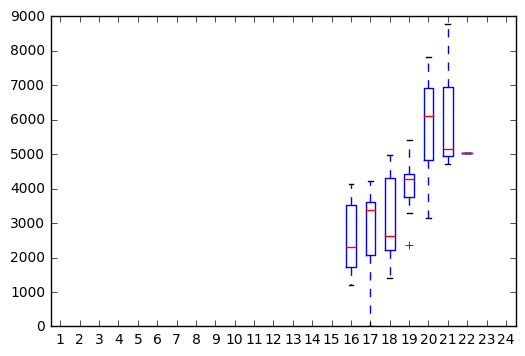
\includegraphics[width=0.4\textwidth]{graphics/noho}
%	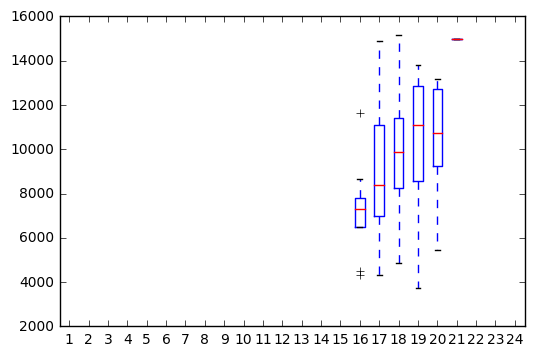
\includegraphics[width=0.4\textwidth]{graphics/sund}
%	\caption{Average throughput of trace (B/s) vs hour of day around Northampton (left) and Sunderland (right). Plots indicate a trend towards higher throughput at night.}
%	\label{fig:tod}
%\end{figure}
%!TEX root = umthsmpl.tex
\chapter{Location privacy threats from advertising services}

In this chapter, I propose to study the possibility of an advertising service to be used for stalking users. I look particularly at stalking entourages and co-travelers.\footnote{We have received IRB approval for this project.}
% This chapter contains mostly proposed work, though it does contain some preliminary evaluations.

Location based services that contain mobile advertisements forward this information on to ad vendors and their clients. These include popular mobile apps such as Grindr and The Weather Channel. An advertiser can purchase advertising through an affiliate, and some affiliates allow for the client to run JavaScript in the ad. As soon as the ad is displayed on one of these apps, the script runs and in some cases sends data to the ad client along with a randomly chosen advertising ID that is unique to the device.

These mechanisms are designed to allow advertisers to target users depending on information such as location. Location information alone can allow advertisers to see where an app is used the most, and target future advertising to those locations. However, simply anonymizing location data does not protect a user from location profiling. De-anonymizing some of these users may be easy, if, for example, the user uses the app at work or at home the majority of the time. While users may trust the application they are using with location information, they likely do not trust advertising clients. As well, this information is rarely restricted by a privacy policy. Most alarmingly, anybody can be an advertiser and target any geographic location for a very low cost.

\paragraph*{Malicious intent}
There are several ways location data obtained from advertising can be used maliciously. It would be very cost effective for an attacker to determine where, for example, gay users are located, by targeting advertising in a certain city and looking at the coordinates located in residential areas of users who used gay-dating app Grindr. As well, attackers could de-anonymize a particular user and target that user to see in realtime their location or predict their location based on history; this would allow them to stalk the user or determine if the user is home. While Grindr has made the sharing of proximity optional to a user, particularly because of privacy concerns\footnote{http://www.grindr.com/blog/grindr-security/}, their location can still be found out by advertisers.

Stalking is a particularly real danger posed by advertising. If a stalker knows where a victim spends a lot of their time, and the victim happens to be using one of the popular apps that are part of the advertising network that the stalker is on, they can be followed. We explore this danger further by quantifying how many users are trackable this easily. We postulate that there are broadly three kinds of users: those who use apps at home for the most part, those who use them in a handful of places, and those who use them in many places. We principally use the advertising identifier (ad-ID) --- a randomly generated pseudonym associated with each user to build an advertising profile --- as ground truth in our experiments.
We specifically look at mobile app advertisements, which are difficult for regular users to block.

We explore also the concept of mix zones~\cite{Beresford:2004}, and how they may both be beneficial and harmful to a person's privacy. On the one hand, a user may want to choose a more populated area to use an app without being de-anonymized. On the other hand, if a person is part of an entourage that does not wish to be stalked, a single person in that entourage could compromise the entire group's privacy by using a privacy-leaking app.

\paragraph*{Experimental design}
To quantify the threat of stalking using an ad service, I plan to verify the following hypotheses.

\begin{enumerate}
\item Users can be seen multiple times, at low cost. We can manipulate how many times each user sees an ad through the bidding settings.

\item There are significant numbers of users who have 0, 1, or 2 \emph{significant stays}. Users with 0 significant stays are nomadic, users with 1 may primarily use their phones at home, users with 2 may be using them at home and work.
% \item There are significant amounts of users in each category of: homebodies, schleps, nomads. Homebodies and schleps are defined as users with 1 or 2 significant stay locations. Nomads have no geographic signature. 

\item It should be fairly easy to identify a user if she has any significant stays. There are two likely scenarios: 1. Consider a person whose details we know about (home, work), and we wish to identify. In our experiments, the identified significant stays serve as a surrogate for the outside information we'd have for the person. 2. Consider a user who has an (ad-ID) initially, and then turns off her ad-ID. Can we de-anonymize a query from that location?

\item Given a list of locations, we can identify nomads by targeting ad-IDs in certain locations. We can validate this by predicting their locations based on a public schedule using information from our advertising logs. 

\item Nomads with anonymous ids may be de-anonymized by cotravelers with de-anonymized ids. We call this the \emph{entourage attack}. This would mean that it is risky to travel in a group, if there are no strict policies on an entourage member's personal device.

\item Users can be targeted and stalked at a low financial cost to the advertiser. The cost is proportional to how easily a group can be targeted, which in turn is proportional to the population with the area of interest.
\end{enumerate}

%% TODO: how cheaply can users / protesters / targets be stalked?

%% TODO: cost?? If target an elected official, how much? How about protesters? How long, how many cities, size of entourage?

%% TODO: don't say Trump

\paragraph*{Preliminary analysis}
The existing dataset contains 350\,000 impressions from 141\,000 users. I validate the first three hypotheses using this dataset. 

% TODO: graph how many users have been subjected to x impressions and delete or change this sentence
\begin{figure}%[p]
	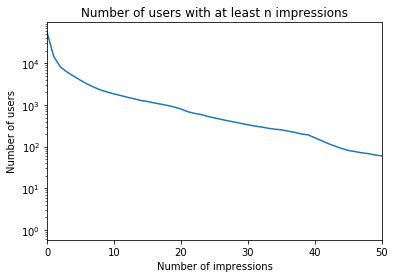
\includegraphics[width=0.5\textwidth]{graphics/numimpressions}
	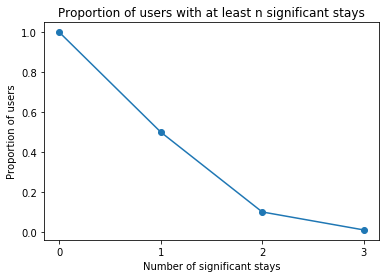
\includegraphics[width=0.5\textwidth]{graphics/sigstays}
	\caption{Left: Number of users with at least $n$ impressions. Right: Proportion of users with 10 or more impressions that have at least $n$ significant stays. }
	\label{fig:impressions}
\end{figure}

\begin{figure}%[p]
	\centering
	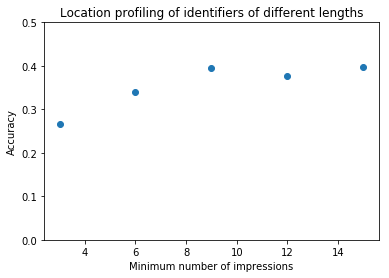
\includegraphics[width=0.7\textwidth]{graphics/impressions}
	\caption{Location profiling accuracy depending on the number of impressions}
	\label{fig:impressionprofiling}
\end{figure}

I first do a survey of types of users in our dataset. 3\% of users have 10 or more impressions (see Figure~\ref{fig:impressions} for more details). Of these users, 50\% are seen at the same one location for at least 3 times a week, 10\% at two locations, 1\% at 3 locations. There are significant amounts of users in the 1- and 2-stay categories. However, 50\% have no geographic signature.
For users with 10 or more impressions, deanonymization based on location is accurate 39\% of the time, testing and training before and after the median times of access. This means even the most naive location profiling methods are effective if we consider significant stays.

% \paragraph*{De-anonymizing identifiers}

\paragraph*{Targeting sports teams}

Despite having no geographic signature in location history, users such as elected officials, celebrities, and sports teams have public schedules. This makes them a viable target for stalking via ads. We target professional sports teams during their active season in 2017. Their travel schedule is public, and relatively unique. As well, there is a cohort of assistants and staff that may reveal the location of the team, whom may want to keep a low profile.

I plan to target NBA and NHL teams in the United States, as well as Premier League teams in the United Kingdom. I build a database of the team's true cities and times from public available information, and target those specific cities for advertising, showing each user the advertisement only once so that travelers are more likely to be reached. I then determine how well advertising identifiers correlate with known location.

There is a risk in targeting sports teams, in that they typically play in large cities, where it is more costly to target tourists or newcomers to the area. If this does not work, I will also attempt to target performers, whom have a public touring schedule and small entourage, but may travel to less populated areas.

\paragraph*{Hiding the identifier}

Users may disable advertising identifiers on their phones. However, users may still be identified by device fingerprinting, depending on the parameters of the advertising network. I plan to look at fingerprinting techniques, including location features, and how linkable they are depending on a user's location. As well, users may be deanonymized by their entourage, which may also help with linking. I also look at the feasability of location profiling co-travelers as a group.

\paragraph*{Summary of proposed work}

I will continue with this work in three directions. First, using the existing ads dataset, I will develop some methods to target users who regularly travel together or meet up. These users would be especially susceptible to the entourage attack. Second, I will collect additional data by targeting locations of sports games to de-anonymize ad-IDs of users who are part of sports teams. Finally, I will target locations of protests for ad-IDs, and follow those ad-IDs to see whether co-travelers can be identified (i.e. whether I can predict the location of someone with no advertising identifier using the location of someone previously physically close to them).

% TODO: use google ads or apple ads instead? better geotargeting?

%\begin{enumerate}
%	\item In the existing dataset, determine whether there are users who regularly travel together or meet up
%	\item In the existing dataset, determine 
%	\item Purchase ads in cities where sports games happen, and determine whether a team can be stalked using the entourage attack.
%	\item Purchase ads where protests are planned to happen.
%	\item Analyze the geolocation risk of apps and events.
%\end{enumerate}
% TODO: risk of using home wifi
%!TEX root = umthsmpl.tex
\chapter{Location privacy without carrier cooperation}
In this chapter, I present methods for users to achieve cell phone anonymity without requiring trust in the service provider\footnote{This chapter is based in part on work published at the IEEE Workshop on Mobile System Technologies~\cite{sung:2014}}. In the preliminary work, I present a GSM-compatible framework that allows for virtual SIM cards so that a user could change her identity regularly. I also present a simple analysis that shows even such a system is susceptible to location profiling, and may not afford the user the desired privacy.

\section{Preliminary work: Anonymous cell phone systems and vulnerabilities}

% Several products exist to 
In this chapter, I prevent several methods a user may pursue to break the link between herself and the cell phone's identifier on the network (i.e. this is an identifier associated with an electronic serial number on the phone or SIM card). These methods are
fully compatible with deployed GSM protocols and infrastructure, from 2G systems typically deployed in poor regions of the world to the new 4G standards deployed in Europe and the US. In our attacker model, we consider carriers that are at best uncooperative, and at worst active adversaries.

\paragraph*{Methods for anonymous cell phone usage}

The most naive method to achieve location privacy is to \textit{anonymously purchase many burner phones}, and use each of them depending on context. 
% TODO: check if these services exist online already
This comes at a high cost, and limits the amount of identifiers a user may have access to. I propose two additional methods: one is a software-based authentication scheme (\textit{ZipPhone}) that requires the cooperation of a mobile virtual network operator (MVNO) that is privacy proactive; the second is a SIM-sharing scheme (\textit{Spartacus}) that allows users to form mix-zones with other users to swap identities.

I plan to investigate the effectiveness of each of these methods, including ease of use, monetary cost, vulnerabilities, and privacy achieved. 

\paragraph*{ZipPhone}
Using a WiFi connection not observable to the cellular 
carrier, a user bootstraps ZipPhone by paying an MVNO for service using an anonymous electronic 
currency~\cite{Ben-Sasson:2014,Miers:2013,Bissias:2014}. Upon payment, the user receives 
one or more IMSIs. This step delinks users and identifiers. 
The user is now ready to use make and receive calls using VOIP. To do so, 
they connect to the GSM network, authenticating themselves with the IMSI, 
which the MNO will verify via signaling to the MVNO (see~\cite{sung:2014} 
for details).

The user periodically discards IMSIs to avoid the gathering  of 
sufficient geographical information by the carrier to classify successfully against 
known profiles of users.  If the user wishes to purchase additional 
ZipPhone IMSIs, they need not necessarily utilize WiFi again. They can 
use their carrier-provided data connection, and contact the ZipPhone 
MVNO using secure protocols over the Internet to do so.

\paragraph*{Spartacus}
A SIM owner can leave an extra Internet-connected phone at their house or other
preferred location (perhaps with the actual SIM) and instruct it to
connect to the network remotely; this setup allows the owner to
reclaim without necessarily revealing their current location. 
Peers that wish to lend out use of their SIM can retrieve the $K_i$
key stored in it (this is done only once), or do a man-in-the-middle attack between the phone and SIM during each remote authentication. They can then
produce the $K_c$ and SRES values for a remote ZipPhone requester, who
can relay via Wi-Fi (or existing cellular connection) the {\em random number} issued by the carrier to the peer during a location update. Keys 
for encryption with GPRS/EDGE also are based on knowledge of $K_i$ and can be similarly relayed.

\paragraph*{Location profiling}
\begin{figure}
	\centering
	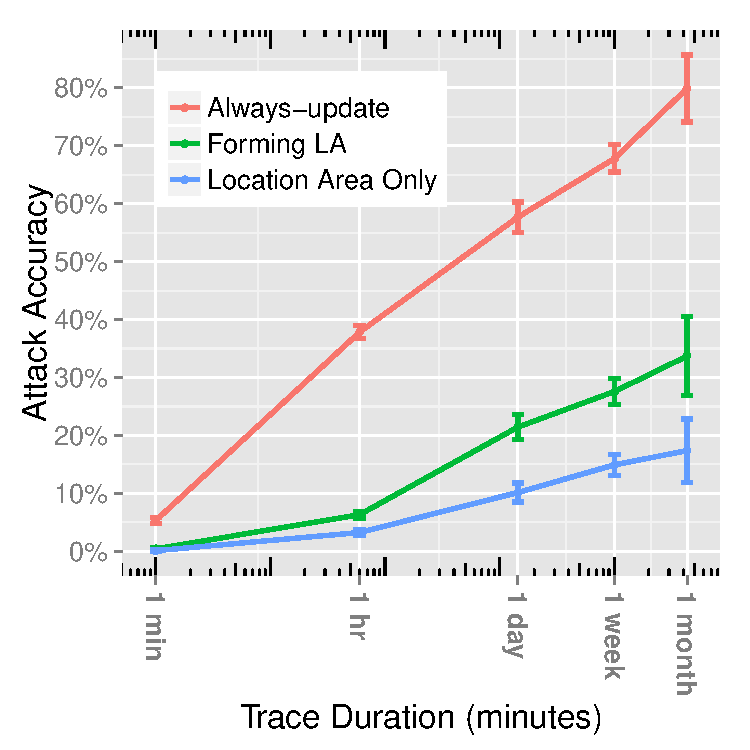
\includegraphics[width=0.7\textwidth]{graphics/mulder}
	\caption{The accuracy of the attack defined by Mulder et al.~\cite{Mulder:2008} under the always-update policy (top, blue line) and forming LA policy (middle, red line). Our results match well with\cite{Mulder:2008}: an attacker achieves a 38\% success rate against users that update their SIM-based identifiers once an hour.  Under the latter, more realistic, forming location area update policy, the attacker's success rate falls to 6\% when SIM-based identifiers are updated once an hour. The bottom, green line shows the lower bound on any scheme: it represents an unrealistic location management scheme where the carrier learns only the location area but not the cell a user is associated with. Errorbars represent 95\% c.i.}
	\label{fig:mulder}
\end{figure}

The effectiveness of the classifier is shown in Figure~
\ref{fig:mulder}. In all cases, the attacker is given a preceding month's 
data as ground truth for training. The blue line is a recreation of results 
from Mulder et al.: a randomly selected  1-month-long sequence of the cells a 
user is associated with results in a high accuracy  of 80\%; Mulder et 
al.\ saw\footnote{These small differences are due to our use of an additional month from the data set.} about 82\%. A random sample of up to 1-hour of cell locations is identifiable 38\% of the time; Mulder et al.\ saw about 44\%. In both cases, random chance would be correct about 1\% of the time. 

% TODO: portknocking
\paragraph*{Fake pages}
In modern GSM networks, phones communicate to specific towers only
when a call (or SMS text or GPRS data packet) is incoming or
originated, rather than whenever a new tower is in
range\cite{Razavi:2011,Wong:2000}. However, a more advanced and
aggressive attacker will proactively cause a phone to communicate with
its nearest tower~\cite{Ficek:2013a} based on an SMS {\em Class 0}
message, ICMP ping, or similar technique.

We can defend against these pages with page-knocking, where the handset answers data pages only after a correct sequence is received (all other pages are ignored). Specifically, the VoIP proxy agree on a  function (e.g., a cryptographic hash) that accepts as input a shared secret key and the current time (in minute granularity). The output of the function is then take one bit at a time: if the bit is zero, no packets are sent (and thus no pages) for $d$ seconds; if the bit is one, a packet (and one page) is sent and then it pauses $d$ seconds. The handset can answer at any time; the proxy doesn't need to know the value $n$. An initial non-empty page is required to start the sequence.

The chances that the carrier can falsify the sequence is $2^{-n}$ for an $n$-bit sequence. The cost is that the user must wait $(n+1)d$ seconds before answering incoming pages for VoIP calls. On Verizon, I have measured $d$ to be $5.12 * 2$ seconds. 

 \begin{figure}[t] 
	\centering{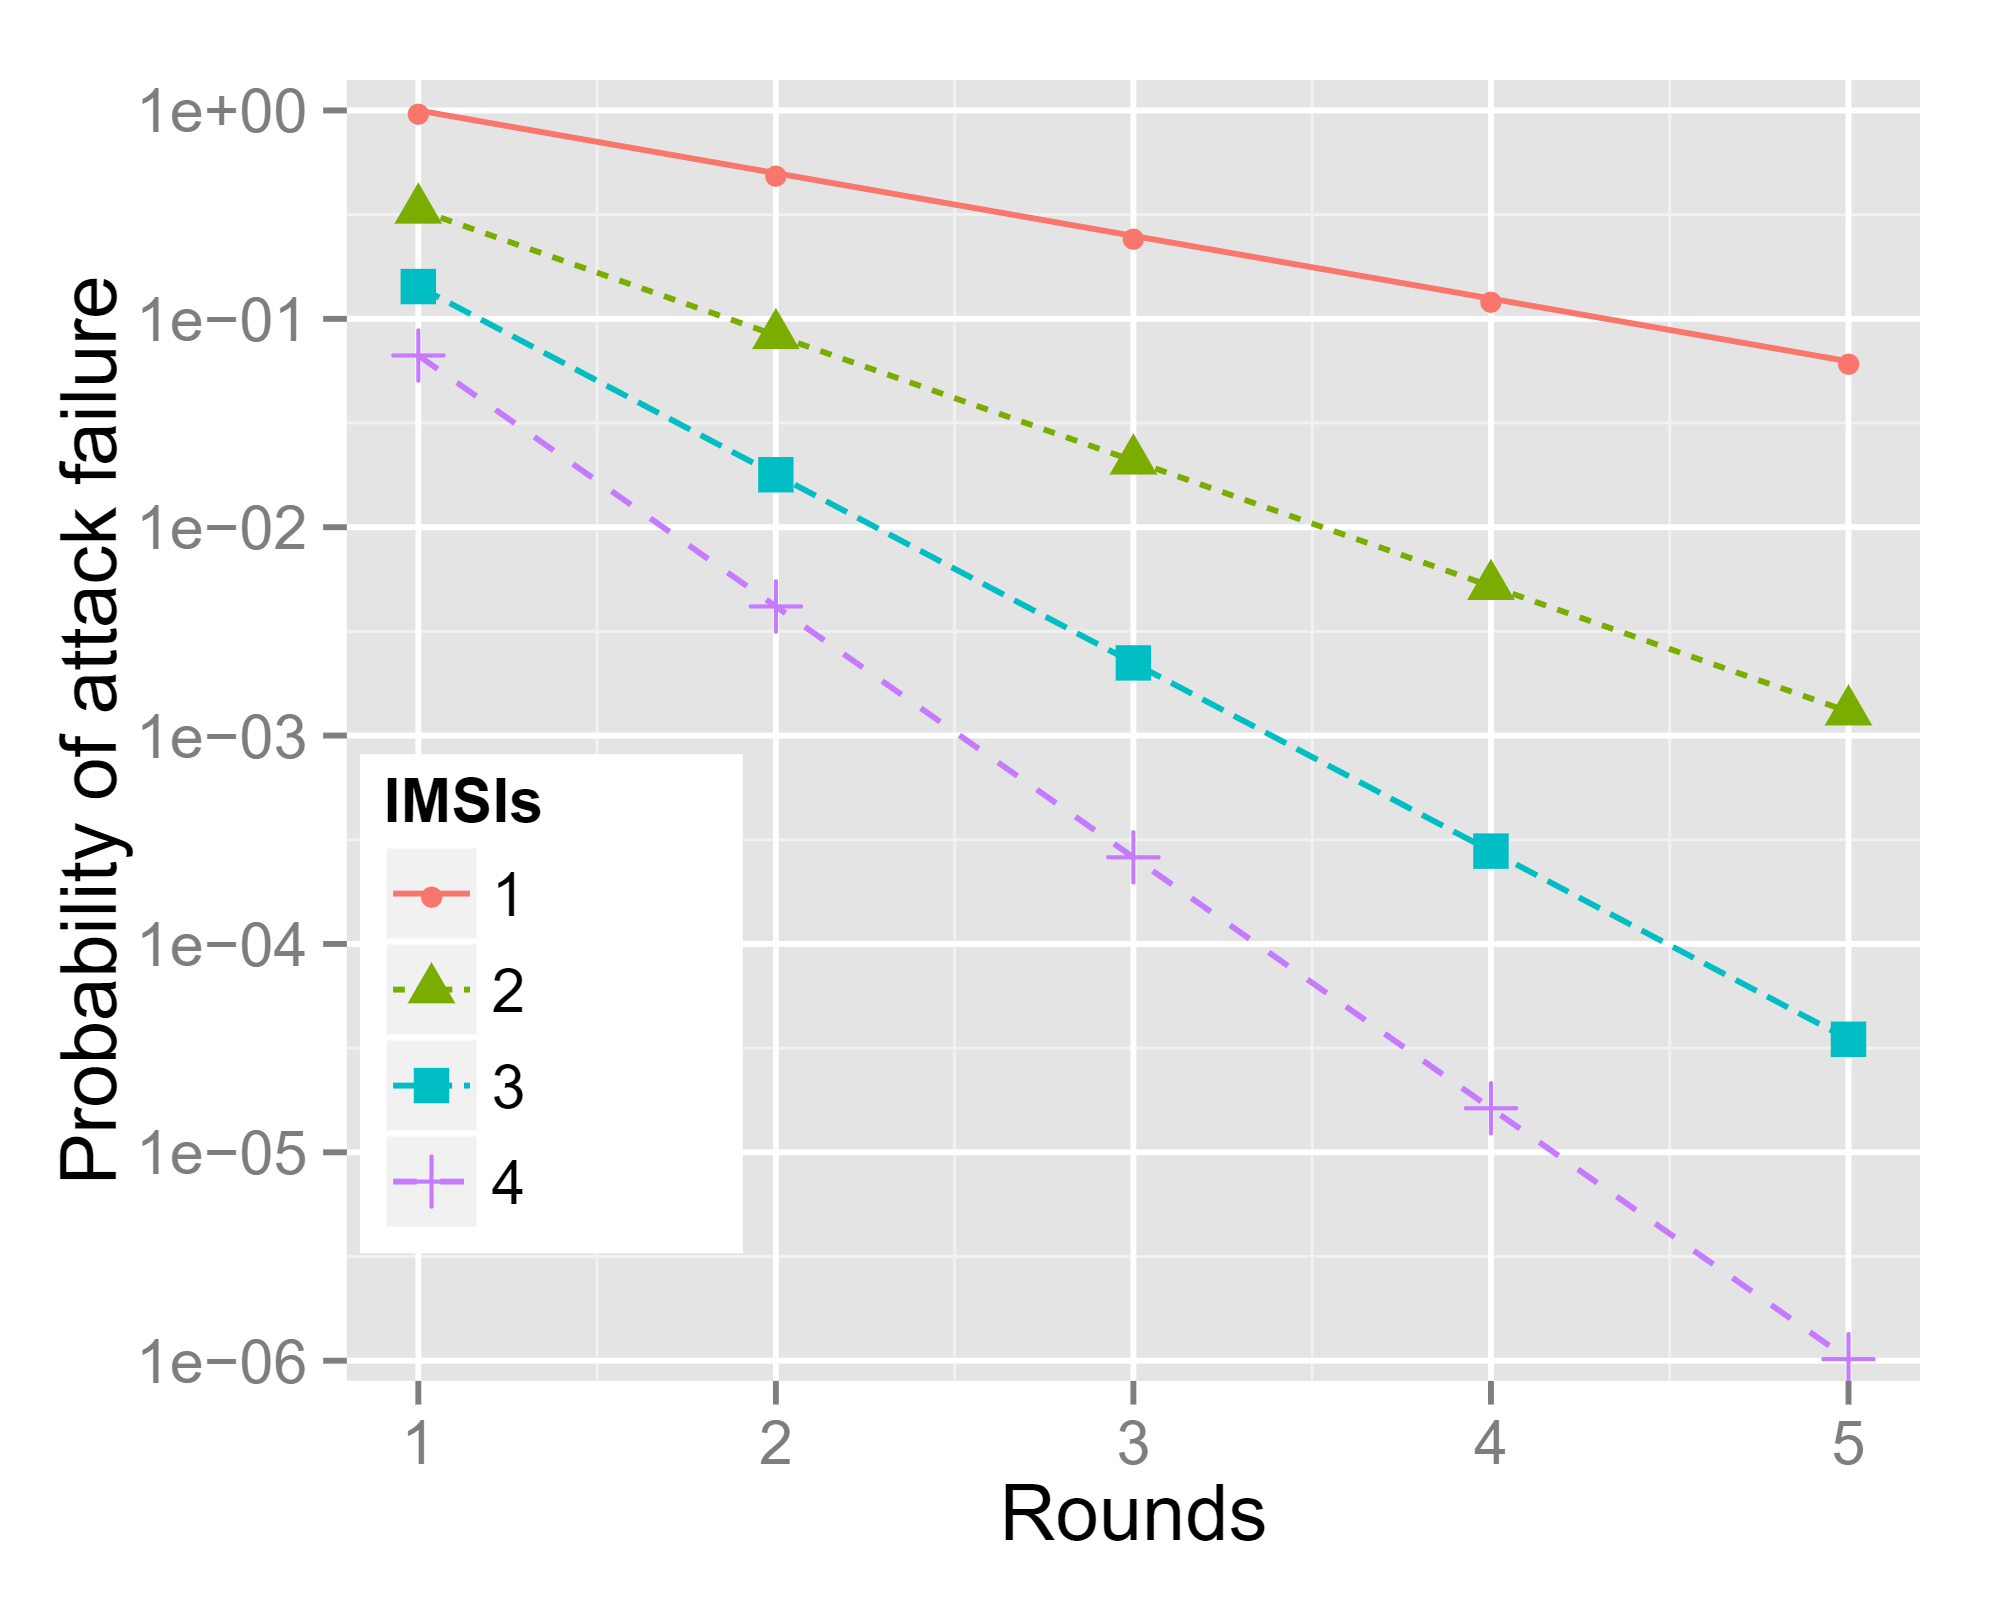
\includegraphics[width=.9\textwidth]{graphics/pageknock} }
	\caption{The probability that an attacker succeeds in crafting a fake page for varying  numbers of rounds $r$ and concurrent IMSIs $m$, based on Eq.~\ref{eq:pk}.}
	\label{fig:pk}
\end{figure}

A more efficient scheme where the phone registers $m$ IMSI values (one at a time)
from a single physical phone, all provided by the ZipPhone MVNO will take about 10--15 seconds to complete. Whenever the
proxy needs to contact the ZipPhone user, it selects a particular
non-empty, unordered subset of the $m$ values, and pages each IMSI
value in that order. Each IMSI can be paged once every 5.12 seconds with overlapping windows. 

For $m$ IMSI values, the number of non-empty unordered subsets for the first round is
$\sum_{i=2}^m{\binom{m}{i}}= 2^m-1.$ Because the empty subset can be included in subsequent rounds, 
for an 
$r$-round  sequence, the probability of the carrier guessing the
correct sequence  is
\begin{eqnarray}
\frac{1}{(2^m-1)(2^m)^{r-1}}. \label{eq:pk}
\end{eqnarray}
Figure~\ref{fig:pk} plots Eq.~\ref{eq:pk}. For example, when $m=3$ IMSIs are
used, the registration delay upon entering a new MSC region is 30--45
seconds. When $r=3$, the probability the carrier can guess the correct
sequence of pages is $0.002$. 

\section{Proposed work}

% TODO: simulate usability issues, simulate usage and trackability
% TODO: PRS and 
Some questions remain from the above work:
\begin{enumerate}
	\item How effective would location profiling and trajectory linking be in de-anonymizing ZipPhone or Spartacus users?
	\item How often would users need to go offline or significantly disrupt usage to avoid tracking?
\end{enumerate}

To answer these questions, I plan to simulate ZipPhone or Spartacus using data collected in Chapter~1. I will evaluate different de-anonymization algorithms, and different methods of evasion.

I will also try to implement Spartacus using SIMTrace hardware and simlabTrace\footnote{https://github.com/kamwar/simlabTrace/wiki}, which is able to sniff and perform a man-in-the-middle attack between the SIM card and phone. This would be a significant engineering effort to implement a modified handshake during the device's attach procedure to the network, and send information between devices.

%I plan to extend the location profiling analysis, as well as implement and evaluate a Spartacus implementation. This includes a trajectory linking algorithm to account for users who deftly try to avoid deanonymization by using different identities based on their location.
%
%\paragraph*{Spartacus implementation}
%To implement Sparatacus, one must perform a man-in-the-middle attack between SIM card and phone. I will investigate the use of SIMTrace and SIMLab to retrieve these credentials.
%
%In sum, I propose the following:
%\begin{enumerate}
%	\item Come up with a billing scheme
%	
%	\item Evaluate location privacy against some dataset or simulated dataset
%	
%	\item Evaluate pageknocking.
%	
%	\item Consider the cost to an attacker to deanonymize
%	
%	\item Investigate methods to estimate the size of a mix-zone.
%	
%	\item Model risk / utility of sharing your SIM with either someone you completely trust, or with a mix of peers that have a probability of turning against you.
%	
%	\item Implement an app that automatically shares an identity, goes dark, requests and identity.
%	
%	\item Implement Spartacus (PeerPhone)
%	
%	\item Test in the field. Evaluate performance and location inference with a mix-zone of 2 with the goal of finding out which new locations a user is visiting.
%	
%\end{enumerate}
%!TEX root = umthsmpl.tex
\chapter{Timeline}
I plan to produce a draft by the beginning of Fall 2017, and defend by the end of that semester. Several significant efforts remain to complete these studies.
\begin{enumerate}
	\item Submit my recent work on throughput localization (Chapter~2) to a journal (March 2017).
	\item Investigate utility and information theory models for location privacy (April 2017)
	\item Find relevant datasets available for academic research and evaluate location profiling and trajectory linking algorithms (May 2017).
	\item Investigate simlabTrace as a way to implement Spartacus (May 2017)
	\item Develop an experiment to evaluate methods of purchasing targeted advertisements based on sports teams and performers, and de-anonymizing users based on information from co-travelers (March 2017).
	\item Data collection of advertisements (March -- June 2017).
	\item Develop a data collection protocol and perform a field survey of Amherst and surrounding area (March -- May 2017).
	\item Synthesize a dataset and evaluate these algorithms using surveyed data (June 2017).
	\item Use the dataset to simulate scenarios for ZipPhone and Spartacus (July 2017).
\end{enumerate}


%%
%% Beginning of back matter
\backmatter  %% <--- mandatory

%%
%% We don't support endnotes

%%
%% A bibliography is required.
\interlinepenalty=10000  % prevent split bibliography entries
\bibliographystyle{umassthesis}
\bibliography{umthsmpl}
\end{document}

%%% Local Variables: 
%%% mode: latex
%%% TeX-master: t
%%% End: 
